\documentclass{standalone}
\usepackage{tikz}
\usetikzlibrary{
  arrows,
  calc,
  decorations.pathmorphing,
  decorations.pathreplacing,
  decorations.markings,
  fadings,
  positioning,
  shapes,
  arrows.meta
}
\pgfdeclareradialshading{glow}{\pgfpoint{0cm}{0cm}}{
  color(0mm)=(white);
  color(5mm)=(white);
  color(9mm)=(black);
  color(10mm)=(black)
}

\begin{tikzfadingfrompicture}[name=glow fading]
  \shade [shading=glow] (0,0) circle (1);
\end{tikzfadingfrompicture}

\ifpdf
% Ensure reproducible output
\pdfinfoomitdate=1
\pdfsuppressptexinfo=-1
\pdftrailerid{}
\fi

\definecolor{atomblue}{rgb}{0,0,1}
\definecolor{atomorange}{rgb}{1,0.483,0}

\begin{document}

% Scale figure so that the text in the final plot is consistent with other figures
% note that the figure size needs to be scaled separately.
\begin{tikzpicture}[scale=1.450]
  \node at (0, 0) {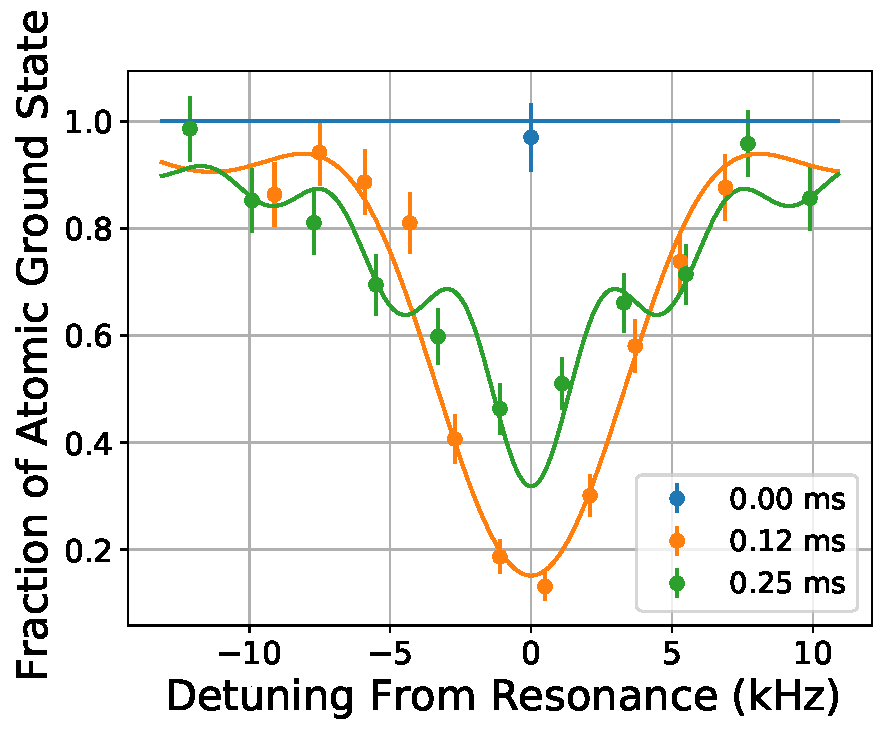
\includegraphics[width=7.71cm]{imgs/exp_data_norm_raman_det.pdf}};
  \node at (-2.3, 1.9) {\footnotesize (\textbf{a})};
  \node at (0, -4.1) {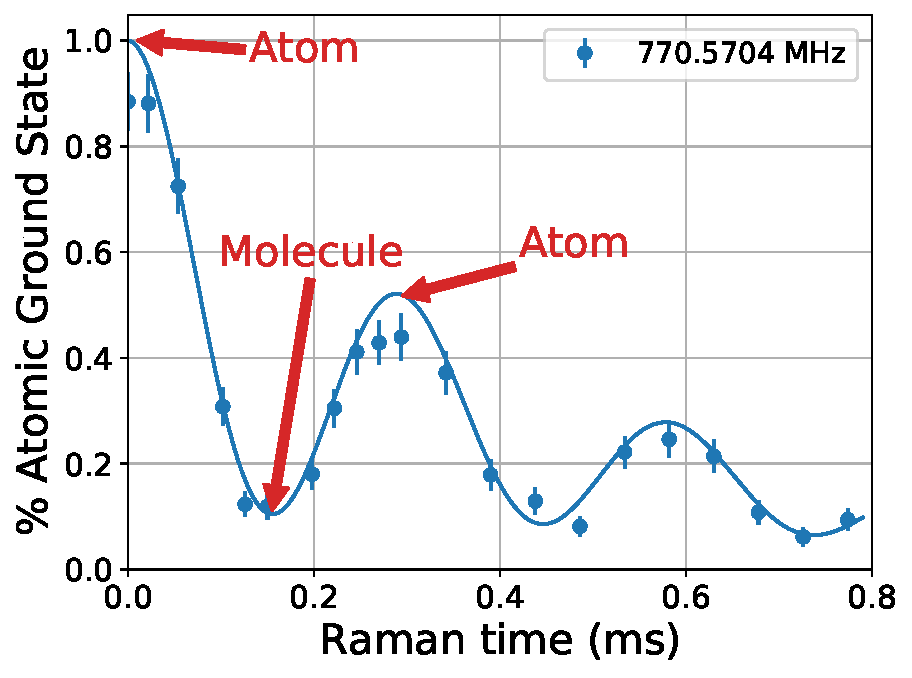
\includegraphics[width=7.71cm]{imgs/exp_data_norm_t.pdf}};
  \begin{scope}[shift={(-1.8, -2.5)}]
    \draw plot[samples=200,domain=-0.2:0.2,variable=\x] ({\x + 0.06}, {\x * \x * 10 - 0.17});
    \fill[atomblue] (0, 0.06) circle (0.075);
    \fill[atomorange] (0 + 0.10, -0.05) circle (0.05);
  \end{scope}
  \begin{scope}[shift={(-0.65, -3.85)}]
    \draw plot[samples=200,domain=-0.2:0.2,variable=\x] ({\x + 0.06}, {\x * \x * 10 - 0.17});
    \fill[atomblue] (0, 0.06) circle (0.075);
    \fill[atomorange] (0 + 0.10, -0.05) circle (0.05);
  \end{scope}
  \begin{scope}[shift={(-1.35, -5.5)}]
    \draw[line width=1] (0, 0.0) -- (0 + 0.15, 0.0);
    \fill[atomblue] (0, 0.0) circle (0.075);
    \fill[atomorange] (0 + 0.15, 0.0) circle (0.05);
  \end{scope}
  \node at (-2.3, -2.1) {\footnotesize (\textbf{b})};
  \node at (0.8, -3.1) {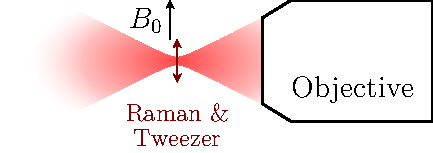
\includegraphics[width=4.80cm]{imgs/apparatus}};
\end{tikzpicture}

\end{document}
